%% ****** Start of file template.aps ****** %
%%
%%
%%   This file is part of the APS files in the REVTeX 4 distribution.
%%   Version 4.0 of REVTeX, August 2001
%%
%%
%%   Copyright (c) 2001 The American Physical Society.
%%
%%   See the REVTeX 4 README file for restrictions and more information.
%%
%
% This is a template for producing manuscripts for use with REVTEX 4.0
% Copy this file to another name and then work on that file.
% That way, you always have this original template file to use.
%
% Group addresses by affiliation; use superscriptaddress for long
% author lists, or if there are many overlapping affiliations.
% For Phys. Rev. appearance, change preprint to twocolumn.
% Choose pra, prb, prc, prd, pre, prl, prstab, or rmp for journal
%  Add 'draft' option to mark overfull boxes with black boxes
%  Add 'showpacs' option to make PACS codes appear
\documentclass[aps,prl,twocolumn,superscriptaddress,groupedaddress]{revtex4}  % for review and submission
%\documentclass[aps,preprint,showpacs,superscriptaddress,groupedaddress]{revtex4}  % for double-spaced preprint
\usepackage{graphicx}  % needed for figures
\usepackage{dcolumn}   % needed for some tables
\usepackage{bm}        % for math
\usepackage{amssymb}   % for math

% avoids incorrect hyphenation, added Nov/08 by SSR
\hyphenation{ALPGEN}
\hyphenation{EVTGEN}
\hyphenation{PYTHIA}

\begin{document}

% The following information is for internal review, please remove them for submission
\widetext
\leftline{Version 1.1 as of \today}
%\leftline{Primary authors: Joe E. Physics}
%\leftline{To be submitted to (PRL, PRD-RC, PRD, PLB; choose one.)}
%\leftline{Comment to {\tt d0-run2eb-nnn@fnal.gov} by xxx, yyy}
%\centerline{\em D\O\ INTERNAL DOCUMENT -- NOT FOR PUBLIC DISTRIBUTION}

% the following line is for submission, including submission to the arXiv!!
%\hspace{5.2in} \mbox{Fermilab-Pub-04/xxx-E}

\title{Investigation of Multi-Mode MHD in Shaped HBT-EP Plasmas}%Electrostatic Feedback on Dipole-Confined Interchange-Turbulent Plasma}
%\input author_list.tex       % D0 authors (remove the first 3 lines
                             % of this file prior to submission, they
                             % contain a time stamp for the authorlist)
                             % (includes institutions and visitors)
\date{\today}


\begin{abstract}
HBT-EP was designed and built to investigate magneto-hydrodynamic (MHD) instabilities that can limit the performance of Tokamak plasmas.  Until the present time, the HBT-EP plasma has been circular in cross section, while the main thrust of research towards a fusion reactor has been redirected toward plasmas that are shaped.  Calculations using the TokaMac and DCON codes predict modifications to the MHD spectrum of a shaped HBT-EP discharge with edge q near resonance - specifically, that the coupling between the unstable and ``most - marginal'' MHD kink modes would be reduced\cite{Maurer}.  This dissertation will investigate the effect by constructing a poloidal field coil which will shape the high field side of the plasma, up to and including imposing a poloidal field null (X-point).
\end{abstract}

\maketitle
%Broad Motivation
\section{Introduction}
The kink mode is a performance limiting, disruptive MHD instability\cite{Strait}.  These modes can be driven by either pressure or current gradients, and HBT-EP has focused on the study of current driven kinks.  The kink mode is present in most tokamaks, including HBT-EP, as the resistive wall mode (RWM) since nearby conducting structural components provide stabilization through eddy currents.  If the wall were superconducting or kink had a high enough rotational frequency and/or a large enough wavenumber in the direction of rotation (n in the toroidal direction, and m in the poloidal), the decay of the stabilizing eddies will be negligible and the mode behavior will approach that of an ideal kink.  In general, of the many possible eigenmodes for the kink, the conditions for instability are that the mode have m and n both as low as possible, with the ratio m/n as close as possible to the average safety factor at the plasma edge (q*).\par
	Shaping in general has been proven experimentally to allow access to higher $\beta$ operating regimes as well as easier access to high confinement regimes (H-mode)\citep{Lazarus, Keilhacker_HMode} while shaping to the point of diversion is necessary to deal with the large heat efflux of a fusion plasma. As such, most modern high-performance Tokamaks operate diverted, as will ITER.  However, multiple codes have predicted a consistent set of effects on the kink mode in a diverted plasma, from a strong suppressive effect on current driven kinks with the growth of a distinct new kink/tearing mode\cite{Huysmans} to a change in the mode-mixing at transition for pressure driven modes\cite{Maurer}.\par
The latter effect can be seen in a current-driven model as well.  Figure \ref{DCON_dW} a) shows how the two least stable mode energies vary with q*, which is varied by changing plasma current, in the presence and absence of shaping.  q* is calculated on HBT-EP using MR and Ip measurements and a circular, cylindrical approximation, which is invalid in the case of a diverted plasma, as seen in b). q* is calculated in this case by using the (1+$\kappa$) correction for an elongated plasma and is seen to be quite different than our equilibrium measurements and circular approximation would suggest.  Mode mixing occurs in limited plasmas at integer q* as the least stable mode changes shape.  We would expect to see a clean mode with a narrow FFT spectrum when the two modes are widely separated, and a mixed mode with a broad spectrum when they come together.  This would be difficult in circular limited plasmas, as both modes are expected to be stable at the crossover.  By contrast, in diverted plasmas, we see that at low current (high q*) there is an unstable mode and a marginally stable mode, which meets the Boozer criterion for n=1 multimode\cite{Boozer}.  Shaping is seen to change the q* values at which the modes exchange stability, and the n=1 multimode region is seen at a q* of ~2.6, rather than an integer value.  Equilibrium values in 2 a) and b) are chosen such that the the plasma is always diverted.  TokaMac and DCON can not integrate to a separatrix, and output, including q* and mode energetics, is seen to be a weak function of how close to the edge the calculation takes place. Fig 2c), however, shows that even in shaped but limited plasmas, i.e. fully simulated to the last closed flux surface (LCFS), the energetics of an equilibrium are seen to vary with shaping.\par
\begin{figure}[htb]
	\centering
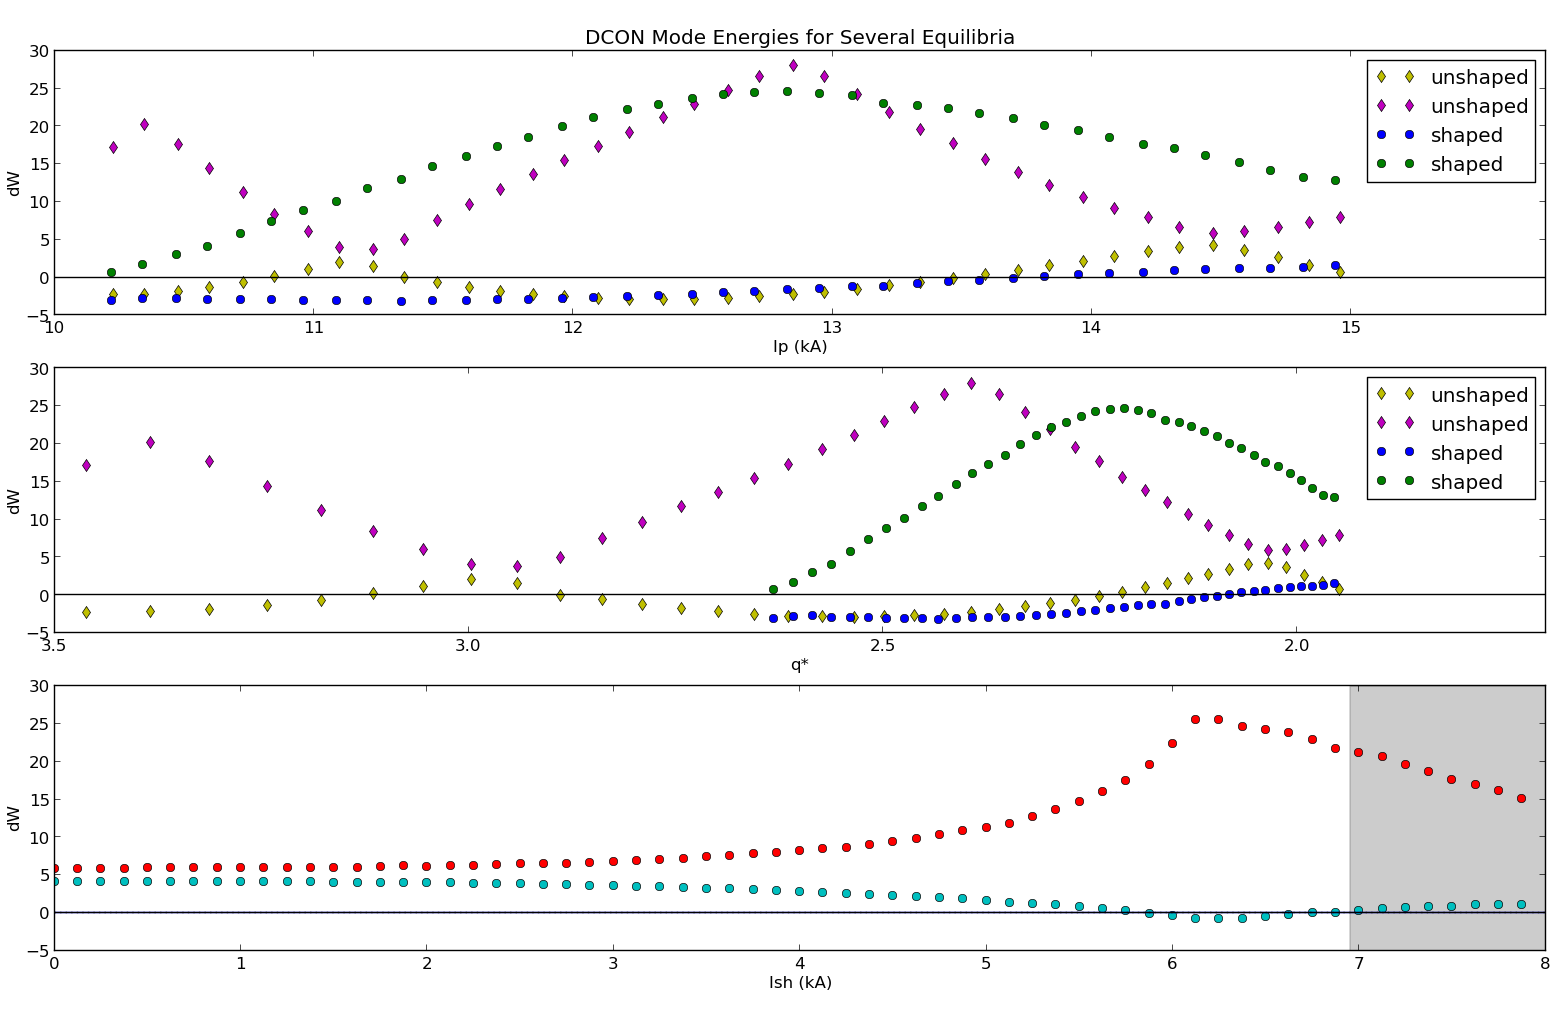
\includegraphics[scale=.2]{../Plots/dW_v_Ip_q_ish_fixed_MR.png}\caption{n=1 mode energies from DCON \\a) dW v Ip, MR = 93cm, Ish = $\frac{8}{15}$Ip\\  b) Same data, plotted against q* with $\kappa$ correction\\c) $MR = 93cm, Ip = 11.1kA$ (unshaped q*=3 resonance in a), plasma is diverted in shaded region, limited in unshaded}
	\label{DCON_dW}
	\end{figure}
	
	\begin{figure*}[htb]
	\centering
	\includegraphics[scale=.25]{../Plots/Plasma_with_sensors_FWall_concept_WithCCview.png}
	\caption{Rendering of the HBT-EP magnetic diagnostics.  Chamber and shell mounted sensor arrays are used to observe and diagnose natural and driven modes MHD.  Passively stabilizing shells and active control coils of various sizes are used to feed back on the modes.  Ferritic sections are retracted for shaping experiments}
	\label{schematic}
	\end{figure*}
HBT-EP is uniquely suited to study the MHD consequences of shaping, as its research mission encompasses the RWM and multimode MHD, and so is well instrumented to detect, analyze and excite MHD activity.  It also has a highly flexible configuration allowing study of MHD in multiple regimes(see Figure \ref{schematic}). It is with this in mind that a zero-net-turns coil similar to those used with success elsewhere\cite{Keilhacker} has been constructed and installed on HBT-EP.  It creates a single null roughly 30${^\circ}$ above the inboard midplane.

	

%Turbulence is a phenomena found in almost every subject involving fluid motion. Turbulence can be either a desired property of flow, such as in a combustion engine \cite{lancaster} (mixing), or a troublesome one, like in the wake formed behind aircraft \cite{spalart}. Plasmas offer an interesting means of interactively studying turbulence as flows can experience forces due to electric and magnetic fields at a distance. In the field of plasma physics, turbulence is believed to play a significant role in the confinement of plasma \cite{wootton, kadomtsev}, generally resulting in a loss of particles, though in some cases is seen to improve confinement \cite{boxer}. 

%Electrostatic feedback has been used as a means to suppress single unstable modes in plasmas \cite{prater, taylor, sen}. Work on the TEXT and KT-5C tokamaks has shown that is it possible to use this same type of feedback to affect the turbulence at the plasma edge\cite{richards, uckan, kan}. Due to the simple magnetic geometry of a dipole confined plasma, the effects of electrostatic feedback can be uniquely studied. The instabilities driving turbulence in these plasmas are low frequency, allowing us to reduce the problem to 2 dimensions with dynamics perpendicular to the magnetic field lines. Greater ease of access with external diagnostic and extended pulse lengths allow the observation of the influence of feedback on a turbulent plasma with substantially increased spatial and temporal resolution compared to previous work, making the dipole geometry an interesting test bed for feedback studies.

%\begin{widetext}

		
%This is a test of twocolumn false
%\end{widetext}

\section{The HBT-EP Tokamak}
\subsection{Present Capabilities}
	For the purposes of this proposal, we will discuss only those diagnostics with immediate relevance to the experiment.  The plasma current (Ip) and major radius (MR) are measured using appropriately wound Rogowski coils, and the loop voltage (LV) by a large Mirnov coil.  At present these, together with the values of our vacuum coil currents, are sufficient to constrain our equilibrium.\par
	\begin{figure}[htb]
	\centering
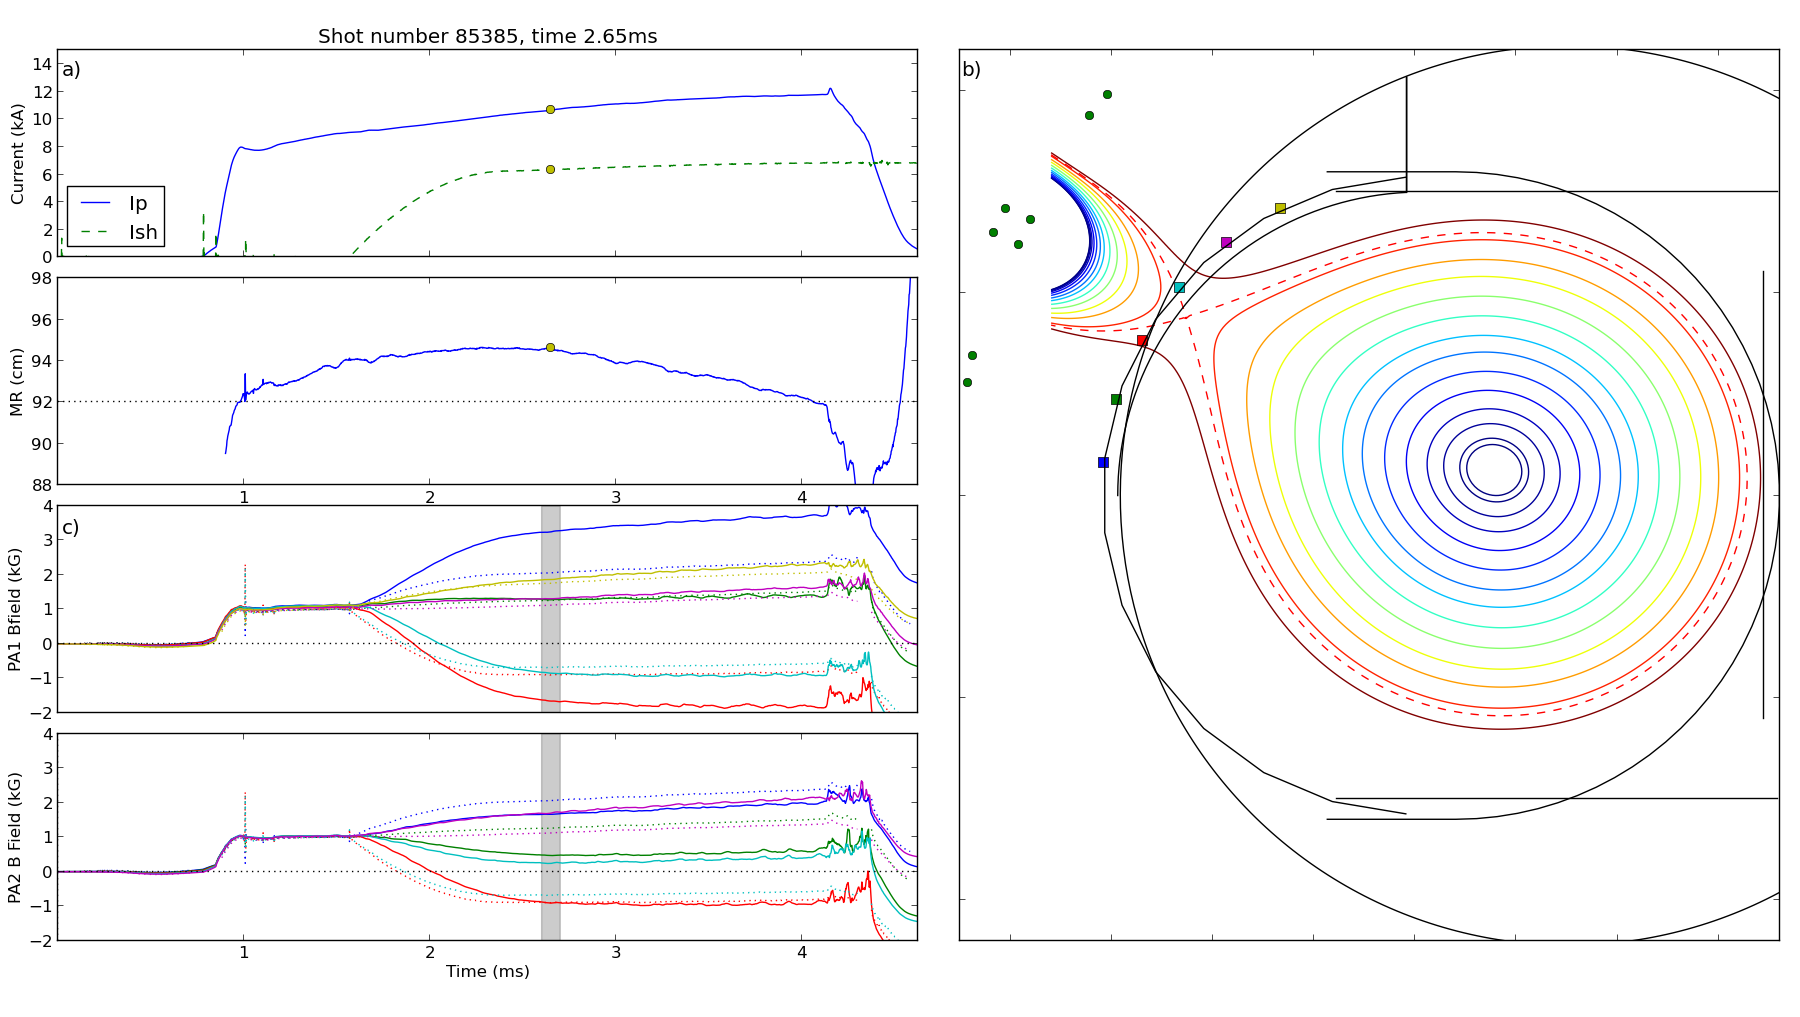
\includegraphics[scale=.1925]{../Plots/shot_85388_currents_fields_fluxes_better_aspect_ratio.png}\caption{HBT-EP shot 85385, including: \\a) Equlibrium measurements of $I_p$, $I_{Shape}$ and MR.\\  b) TokaMac equilibrium reconstruction of flux surfaces\\c) Sensor measurements of Bp near the x-point, compared to expected values (dotted lines).  Sensors locations are shown in b), traces are color coded to their sensor.\\}
	\label{fluxes and fields}
	\end{figure}
	Furthermore, HBT-EP has recently been instrumented with a 2J, 10ns Thompson scattering system, which will allow 3-point profiles of temperature and pressure in the near future.  It is also intended to upgrade the system further, to allow a 10-point measurement, but this may take place after the proposed work has been completed, and 3 points should be more than sufficient.\par
	Twenty stainless steel shells are used to passively control magnetic fluctuations (Figure \ref{schematic}).  Each shell is further instrumented with 3 independent sets of 2 actively driven saddle coils, allowing excitation or suppression of natural modes in the plasma.  216 Mirnov coils, arranged toroidally and poloidally in a high density array (green, blue, and red rectangles in Fig. 2), are used to measure equilibrium fields, fluctuations in the field, and responses to externally driven perturbations.\par
	Figure \ref{fluxes and fields} shows a reconstructed shaped equilibrium.  The measurements of $I_p$, MR, and shaping current ($I_{sh}$) at 3ms, shown in a), are fed into the TokaMac equilibrium code, and the resulting flux surfaces are plotted in b).  Measurements of the poloidal field from sensors near the x-point are displayed in c), along with dotted lines representing the expected field from the equilibrium.  Qualitative agreement is seen, and the discrepancies will be discussed further in the Potential Issues section.\par
	Fluctuations are separated from the equilibrium signal by a 3-pass "hasystack" boxcar smoothing algorithm, and the results, shown in Figure \ref{Stripey_85385}, clearly show the structure and dynamics of the mode activity in the plasma as it evolves.  The fluctuations are then subjected to a Singular Value Decomposition (referred to in the literature as 'biorthogonal decomposion' or 'BD'\cite{de Wit}) to find coherency in space and time, isolating the multiple modes of oscillation.  This allows for the discrimination of higher order, lower amplitude modes.  The appropriateness and utility of the BD for analyzing magnetic fluctuations on HBT-EP has been thoroughly investigated\cite{Levesque}, and so will be taken for granted in this paper.\par
\begin{figure}[htb]
\centering
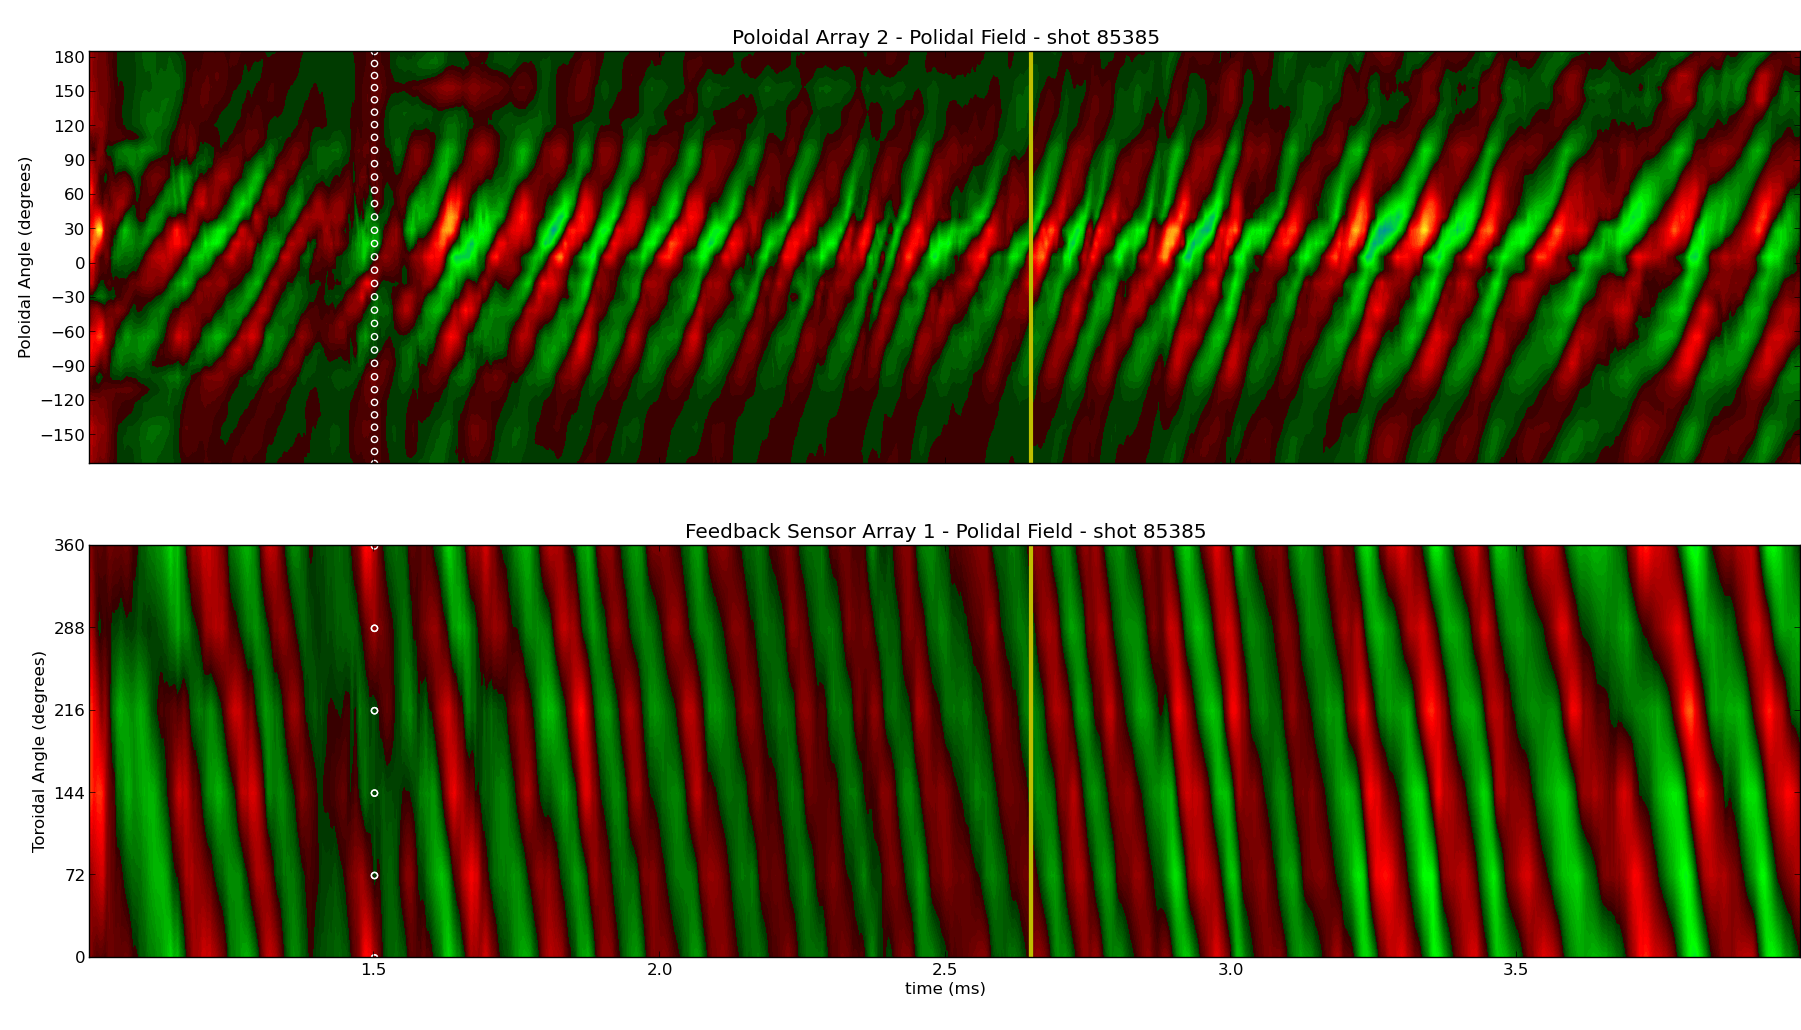
\includegraphics[scale=.2]{../Plots/stripey_plot_85385.png}\caption{Poloidal and Toroidal contours of perturbed poloidal field $B_\theta$ in shot 85385.  Sensors located at white circles.\\m=3, n=1 structure is visible at the time of equilibrium reconstruction (yellow line)}
	\label{Stripey_85385}
	\end{figure}
	We are concurrently performing studies of the effects of ferritic material on the plasma, and so those shells will be retracted and signal from sensors mounted to ferritic shells (gold panels in Fig. 2)  will be excluded from analysis in the experiment.  This reduces to 178 the number of usable sensors, which is still a large multiple of most experiments' resolution.
	
\subsection{The HBT-EP Shaping Coil}
    We will shape HBT-EP plasmas using a quadrupole poloidal field coil positioned outside the vacuum vessel, at the inboard side of the torus, just above the midplane.  The coil is a single continuous conductor wound in both the co- and contra-IP direction forming a 'zero-net-turns' divertor similar to that used in ASDEX-Upgrade\cite{Keilhacker}.  The coil's field decays rapidly in r and $\theta$, ensuring that the shaping of the plasma is highly localized in radius and poloidal angle.  Due to this the coil required construction as close as possible to the plasma, inside the TF coils and just outside the inboard edge of the vacuum vessel (see Figure \ref{Coil_HBT_Section}).\par
This coil is powered by a two-stage capacitive power bank, similar in operation to those used to power HBT-EP's other electromagnets\cite{Gates}. A low capacitance, high voltage startup supply discharges quickly to initialize the pulse, and a high capacitance, low voltage crowbar supply sustains the discharge current for the life of the plasma.  As seen in Figure \ref{fluxes and fields}, the shaping pulse is nearly constant in time - though the capability exists to have it ramp slowly with $I_p$ - and is a significant fraction of the plasma current.  The crowbar bank is passively switched into the system through a diode, greatly simplifying the construction and control of the bank, and ensuring a smooth discharge shape as the bank switches in.
	
\begin{figure}[htb]
	\centering
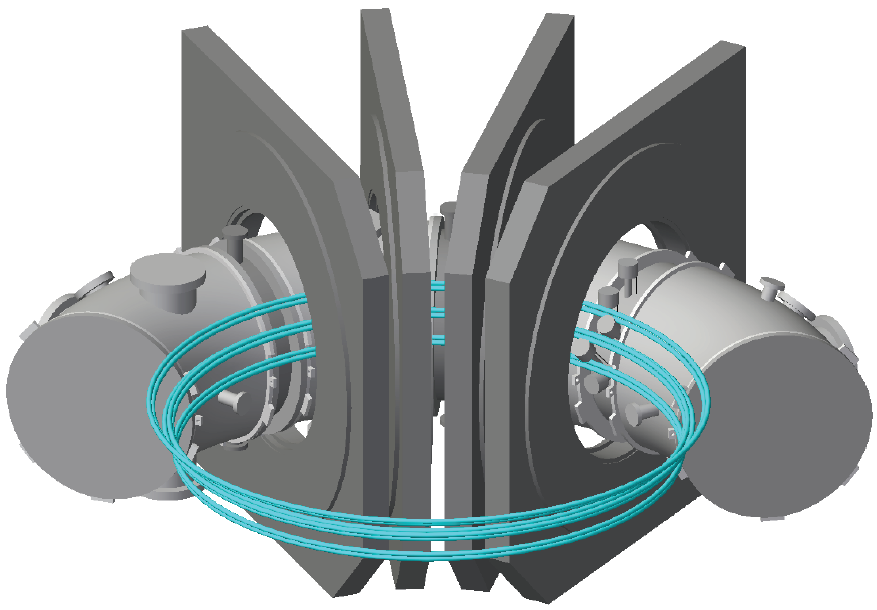
\includegraphics[scale=.35]{../Plots/HBT_section_cropped.png}\caption{Section of HBT-EP, shaping coil shown in blue}
	\label{Coil_HBT_Section}
	\end{figure}
\section{Proposed Research}
	This document proposes to study the structure and dynamics of the shaped MHD spectrum, in the presence or absence of resistive stabilization of the plasma and/or resonant magnetic perturbations (RMPs).  The shaping coil current will be varied to allow observation of diverted plasmas as well as shaped limited plasmas, allowing detailed comparison to calculations of the effects of shaping, and to determine if the effects, if any, lie on a continuum or whether the imposition of an X-point creates a bifurcation in the plasma's behavior.\par 
	\subsection{Natural Modes in Circular Limited, Shaped Limited, and Diverted Plasmas}		
	The coil has a fast turn-on and a slow RC decay, allowing a constant shaping field to be imposed as rapidly as the wall-time of the chamber will allow.  This field can be chosen in concert with the plasma equilibrium to ensure a diverted plasma throughout an individual discharge, though the volume of the plasma, and consequently the wall coupling, will change with $I_p$ and MR.  Slightly more difficult, but still well within our capabilities, would be choosing initial conditions for the power supply such that the shaping current will rise proportionately with the plasma current, thus keeping the location of the last closed flux surface and X-point, if the plasma is diverted, relatively fixed in space.  This would allow us to observe the modes in shaped and/or diverted plasmas with a roughly constant cross-sectional shape, as we currently do with circular plasmas.\par
	Modifications to the poloidal structure of the modes have been observed already.  This is seen in Fig. \ref{Stripey_85385}, near $+150^{\circ}$.  The shaping coil's ramp-phase lasts from 1.5 to 2.5 ms, and residual pickup is indeed seen in the raw fluctuations at this time.  However, the boxcar smoothing rapidly improves as the shaping coil maintains its steady state value, and at 3.5 ms, there is a clear 'hitching' as a mode trough passes that area, with the peak eventually passing in a rapid, high amplitude spike.  The mode is seen to continue rotating far away, giving the appearance of the poloidal perturbation 'piling up' at the x-point as it rotates.\par
	Not enough analysis has been done to say definitively what is occurring.  It is unlikely that the X-point is exerting a poloidally localized torque on the mode.  It is however possible that there is a second mode, highly localized at the X-point, which is interfering with the dominant mode.  Locking to error fields, which are significant (see Potential Issues below) is another factor that must be considered.  Either or both of those options could be consistent with the X-point localized kink/tearing mode\cite{Huysmans}
	\subsection{Effect of Resistive Wall Stabilization on natural MHD Modes}	 
HBT-EP's modular walls will be retracted or inserted to influence the amount of passive stabilization of the MHD modes.  Retracting the shells, one would expect to see the unstable MHD modes appear with faster growth rates and, possibly, larger amplitudes\cite{Shiraki}.  This should help discriminate the unstable modes from the more stable fluctuations and increase the contrast between the observed modes and background noise.  Our walls are designed to be conformal to a circular plasma, and will thus have reduced coupling to a shaped one, but assuming a shot can be developed with a constant position and shape as the shell radius is varied, we should be able to draw comparisons.  With the ferritic segments installed in the vacuum vessel, we will only be able to use 10 of the 20 shells for this experiment, but that should provide enough stabilization to discern a difference.\par
	\subsection{MHD Response to Driven Perturbations}
HBT-EP's active control saddle coils will be used to impose RMPs of varying helicities to investigate the sensitivity of a shaped or diverted plasma to resonant and non-resonant perturbations.  This has been investigated in circular plasmas previously\cite{Shiraki}.  As seen in Fig \ref{Shiraki_plot}, the 3/1 content of the mode is the major factor in determining plasma response.  Whether the level of response to an RMP's 3/1 component increases or decreases, or whether the response will couple more strongly to a different helicity altogether, and how these effects vary with q* will be the main thrust of this experiment.\par
	
\begin{figure}[htb]
	\centering
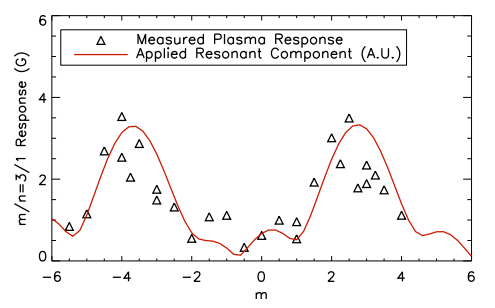
\includegraphics[scale=.525]{../Plots/Shiraki_thesis_Fig_7_1.png}\caption{Plasma response to RMPs of various helicities.  The red line represents the relative amount of +3/1 helicity in each mode.  Taken from referenece \cite{Shiraki}, Figure 7.1}
	\label{Shiraki_plot}
	\end{figure}
%	The plasma will be shaped with a variety of shaping coil pulses. To begin with, a 'flat-top' current pulse has been used to impose a steady, constant shaping field.  A large database of these shots has been created and is in the process of being analyzed.  The field imposed will be large enough to ensure diversion throughout the development of the plasma during its lifetime, though the location of the X-point will vary.  Subsequently, we will attempt to develop a discharge and shaping pulse in order to ramp the current in such a way that the plasma is strongly diverted and the location of the X-point will hold relatively constant.
%We have taken shots with the stabilizing shells both fully inserted and retracted before the installation of HBT-EP's ferritic wall segments.  Post installation, we can still retract all segments, but will only be able to insert the 50\% of the shells with no ferritic attachments, in the interest of reducing the variables in the experiment.\par
%We also intend to take shots with RMP's of various shapes and amplitudes imposed by the control coils.  The response of the plasma to these RMP's will be compared to a circular plasma.  As the coils are mounted on the shells, we will only be able to use half of the normally available coils.  This will reduce the strength and fidelity of the RMP we can impose, and will require us to gather data on circular plasmas with this configuration rather than using existing data from our complete array.  It should still be possible to determine the nature of the differences between a shaped and circular plasma, and quantify them to some extent.\par
%The existing HBT-EP suite of data analysis software, in particular biorthogonal decomposition of our magnetic sensors, will be used to examine the visible MHD modes.  In general 2 modes are clearly visible, though occasionally 3 can be discerned simultaneously.  The relationships between the dominant and sub-dominant modes will be analyzed with regards to their absolute magnitudes, their magnitudes relative to one another, their rotational velocity, and their geometry in the presence and absence of shaping.

\section{Preliminary Findings}
	Several runs have been dedicated to the shaping coil since construction was finalized.  We have shaped the plasma in the presence of a variety of configurations of our passively stabilizing conducting walls, and in the presence and absence of actively driven resonant magnetic perturbations (RMPs).   Unfortunately, a lack of proper calibration at the time of data acquisition means that they are not well categorized, but we have used this work to fine-tune our analysis code, determine the safe operating parameters and determine deviations from the design. \par 
		
\begin{figure}[htb]
	\centering
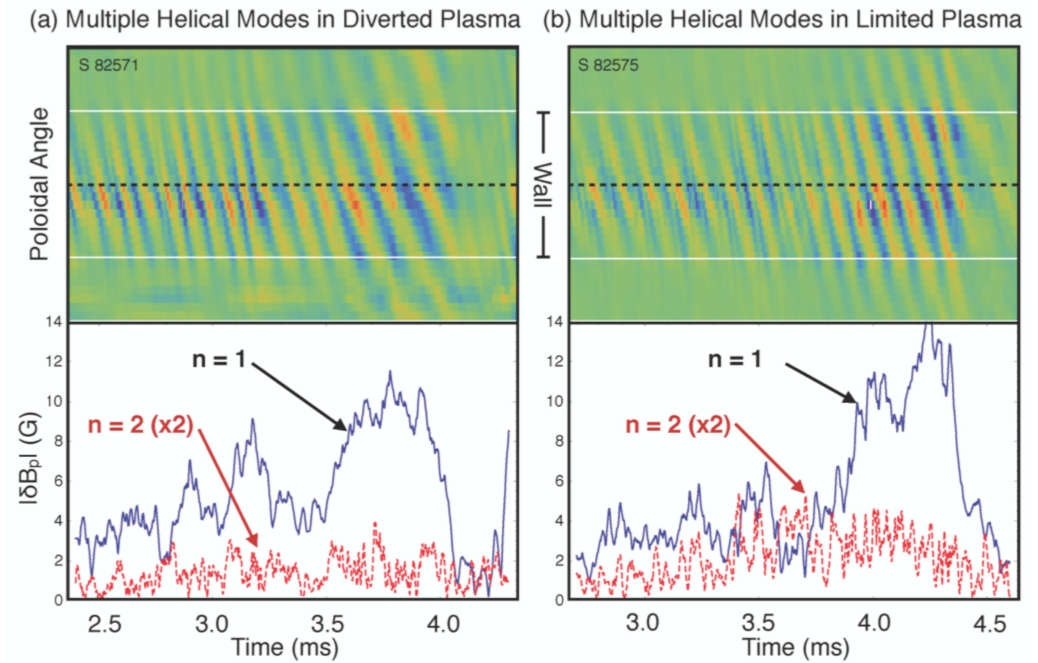
\includegraphics[scale=1]{../Plots/IAEA_plot_cropped.png}\caption{Mode content for shots 82751 (plot label is a typo) and 82575.  n=2 content is seen to be lower relative to n=1 in a shaped plasma}
	\label{IAEA_plot}
	\end{figure}
\begin{figure}[htb]
	\centering
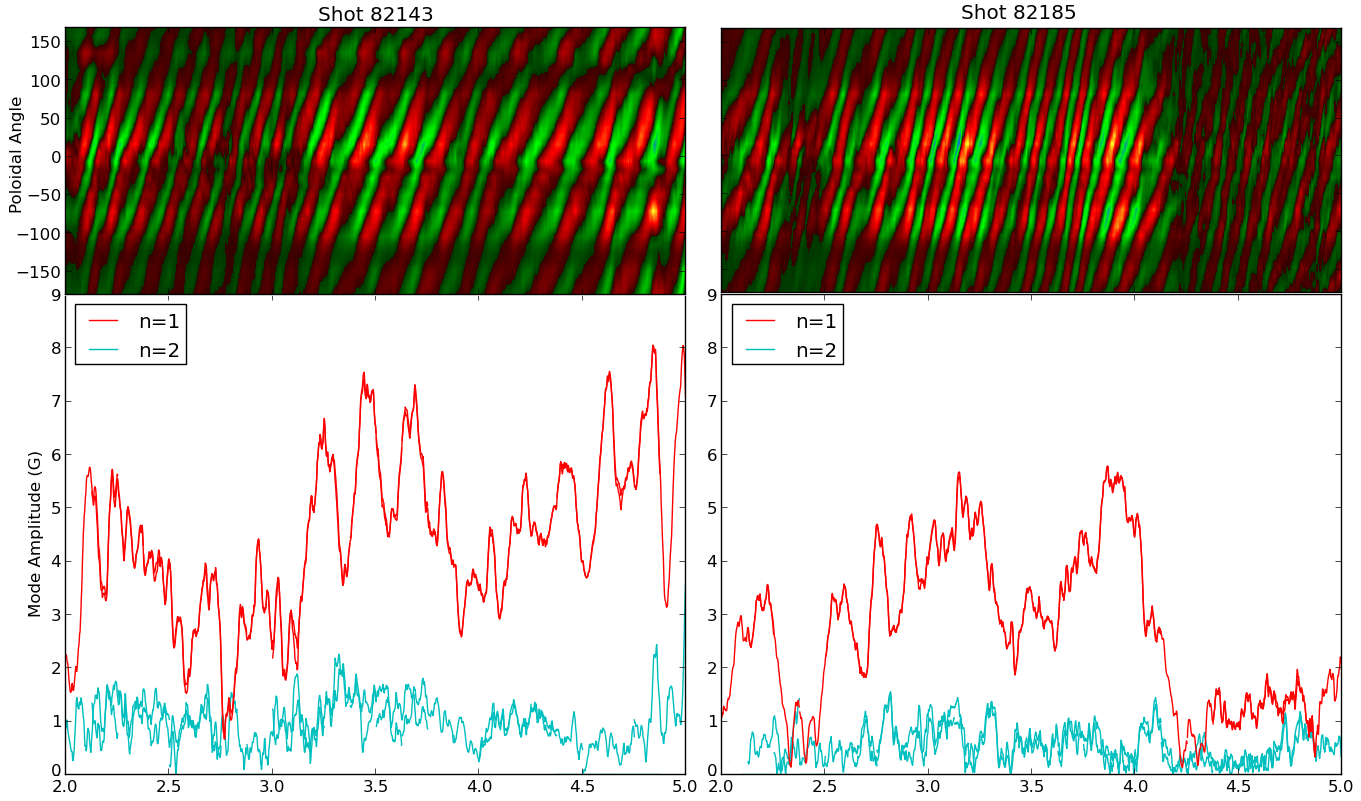
\includegraphics[scale=.25]{../Plots/82143_82185mode_amp_stripes.png}\caption{\\Mode content for shots 82143 (shaped) and 82185 (unshaped).  n=2 content is seen to be higher in a shaped discharge.}
	\label{Modes_stripes_143_185}
	\end{figure}

	Thus far, the observed multi-mode behavior has followed no clear pattern.  Two pairs of shots that have been analyzed illustrate this.  Shots 82751 and 82575 are analyzed in Figure \ref{IAEA_plot}.  Contours of the plasma fluctuations in the poloidal arrays show a dominant 3-1 mode, while a (5 or 6)-2 mode can also be distinguished.  The shaped plasma seems to have the n=2 mode suppressed, while the main n=1 mode seems to rotate faster, up until the slowdown that precedes a disruption.\par
	Shots 82143 and 82185 have different behavior, as seen in Figure \ref{Modes_stripes_143_185}.  These shots are more closely located in time, meaning chamber conditions and background pressure are likely more similar than the other pair.  MR and Ip behavior also agree more closely through the shot lifetime.  In this pair we also see the shaped plasma speed up after shaping is imposed at 2ms, slowing down again around 3ms.  However the mode in the unshaped plasma is rotating much faster than in the previous set.  We also see the n=1 mode much stronger in the shaped plasma than the unshaped, and the n=2 mode may be excited as well.  The n=1 crash in the unshaped shot correlates with edge q going above three, in agreement with theory, while the shaped plasma shows no such behavior.\par
	The main lesson of these two shots is that HBT-EP's intrinsic shot-to-shot variability will require a large dataset, gathered in as small an interval of time as possible, to ensure that meaningful conclusions can be drawn.  During the next run campaign, replicating these shots will be a top priority.\par
	\begin{figure}[htb]
	\centering
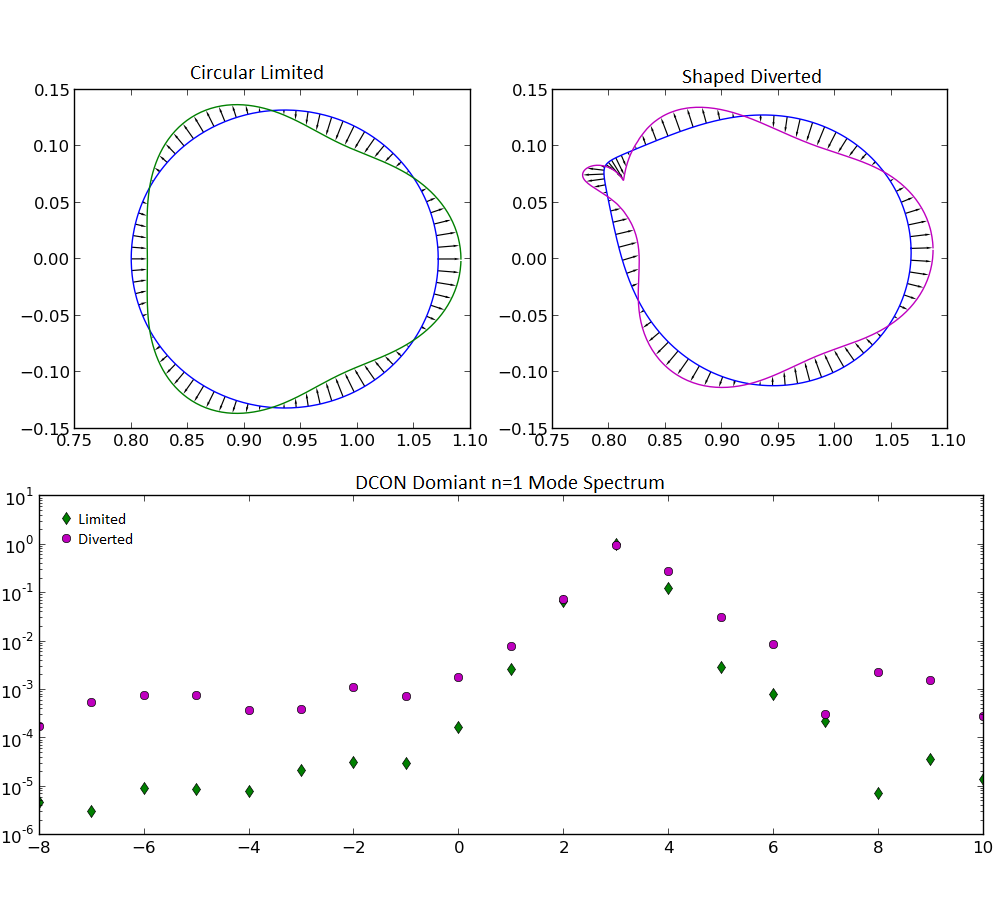
\includegraphics[scale=.35]{../Plots/Dcon_surfaces_n1_dom_85385_85402.png}\caption{DCON predicted mode structure and Fourier spectrum for shot 85385 (w/ \& w/o shaping current) at 2.65ms (see also Figs \ref{fluxes and fields} \& \ref{Stripey_85385})}
	\label{DCON_mode_structure}
	\end{figure}
	
	\begin{figure}[htb]
	\centering
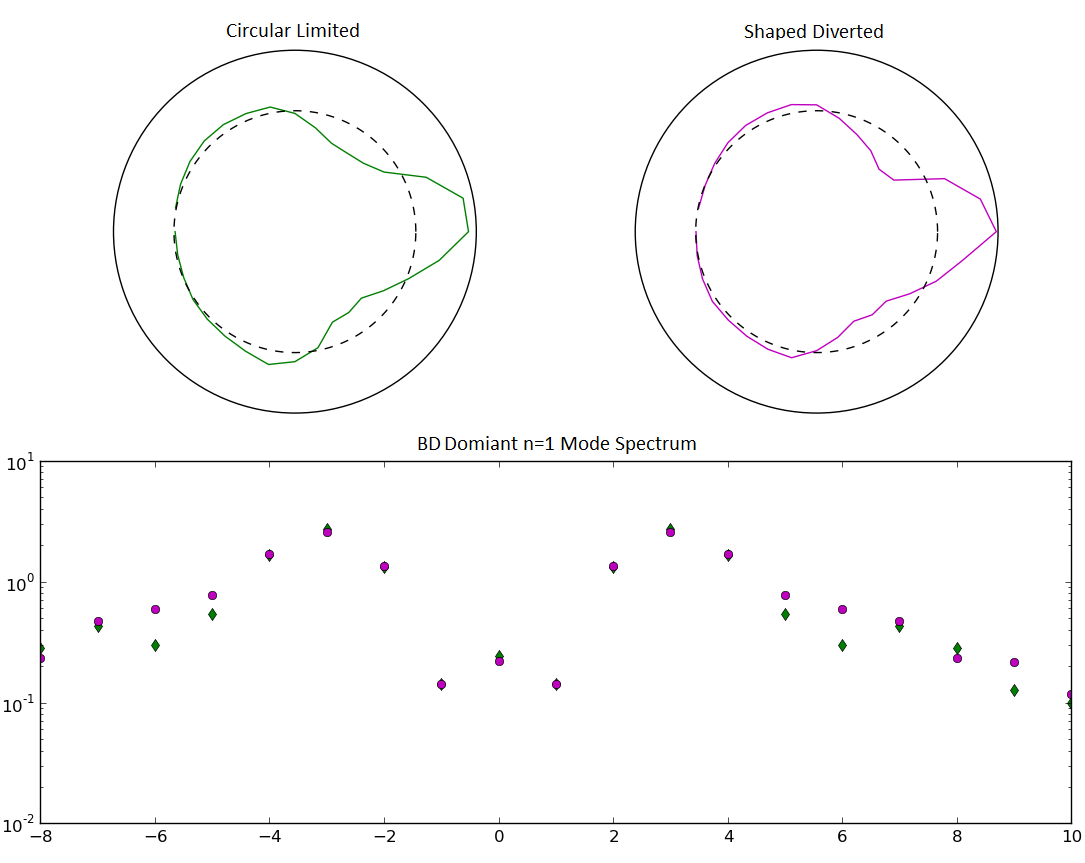
\includegraphics[scale=.3]{../Plots/BD_surfaces_n1_dom_85385_85402.png}\caption{BD breakdown of measured mode structure and Fourier spectrum for shot 85402(unshaped) and 85385 at 2.65ms (see also Figs \ref{fluxes and fields} \& \ref{Stripey_85385})}
	\label{BD_mode_structure}
	\end{figure}
	
	DCON has also predicted large changes in the natural mode structure of a shaped plasma, as seen in Figure \ref{DCON_mode_structure}.  Over and above the deformation caused by overlaying the mode on a shaped equilibrium surface, we can see that an extra zero-crossing is introduced near the x-point, and that the poloidal mode spectrum is broadened.  Direct measurements of the main n=1 mode in the plasma on which the DCON calculations are based are less conclusive (Figure \ref{BD_mode_structure}).  However, measured mode amplitude at the point of interest is limited by several factors, including the more rapid attenuation of high-order components of the mode, the outboard position of the current baseline shaped HBT-Equilibrium, and the variable sensor coupling at the location of interest due to the non-circularity of the plasma.  Forward modeling of test cases in Valen to determine the expected sensor pickup on these modes should help us to understand this effect.\par
	Due to the construction of the physical coil concluding months before the creation of a suite of reliable analysis code, ensuring diversion has been unreliable.   However, the plasmas are definitely shaped, several are diverted, and the mode spectra characteristics of shaped plasmas have not been seen to change significantly from a circular, limited plasma.  This is surprising, but encouraging, as it would mean that much of the MHD work that has been and is being done on circular, limited plasma experiments is of direct applicability to the more advanced tokamaks.  More careful design of experiments, and finer data analysis, performed concurrently with data gathering, will enable us to increase the period of time in which the plasma is diverted.

\section{Potential Issues}
	The shaping coil was installed in-situ, without disassembling the machine first.  This added to the complexity of installation and required certain compromises in the design.  The coil itself was constructed of highly flexible welding wire to ease installation, but the lack of rigidity leads to motion of the coil during a shot.  This effect has been studied, and the motion is less than 0.7mm during the lifetime of the plasma.\par
Secondly, the thickness of the welding wire, the lack of space and high density of external ports and other obstructions on the high field side of the machine have made threading the coil in an axisymmetric manner impossible.  The effects of this were expected to be small, however, large differences between the measured fields on the toroidal array sensors and the two poloidal arrays, as seen in Figure \ref{fluxes and fields}, suggest that the errors were larger than anticipated.  Work is ongoing towards understanding and minimizing these errors.\par
Regardless, the spatial deviations all tend to be in the direction of increasing the coupling between the coil and plasma.  This is better than the alternative, as the X-point acts as a physical limiter.  At the toroidal location where the shaping is strongest, material that lies outside the local LCFS will run to the wall and be scraped off, even if it would be within a confined plasma elsewhere.  The result is a plasma that is generally more strongly diverted than otherwise.  If the intent is to only apply a low level of shaping, the same argument applies, and it should be possible to achieve our ends by recalibrating the shaping current to account for the fact.

\section{Acknowledgements}
Design, fabrication and installation were all aided greatly by the contributions of Nick Rivera and James Andrello.\\
%\begin{figure*}[htb]
%	\includegraphics[scale=.25]{Thesis_Proposal/Plots/Plasma_with_sensors_FWall_concept_WithCCview.png}
%	\caption{Rendering of the HBT-EP plasma with instruments. Passively stabilizing shells and active control coils of various sizes are used to feed back on MHD modes.  Chamber and shell mounted sensor arrays are used to observe and diagnose natural and driven modes}
%\label{schematic}
%\end{figure*}
%\onecolumngrid
%\twocolumngrid

%Concept
%In this Letter, we present the results of the first application of electrostatic feedback in a dipole confined plasma. By measuring fluctuations of the floating potential and applying these fluctuations, phase shifted and amplified, to the plasma (via current probe) we measure an influence on the turbulent spectrum, both amplification and suppression depending on phase. In contrast to previous experiments, we observe the influence of this feedback across magnetic field lines. We note a clear dependence on the orientation of the sensor-actuator arrangement with respect to plasma rotations, displaying a decorrelation of the the signal from the actuator with azimuthal angle. A linear model of the pressure driven interchange mode including the feedback system predicts much of the measured dynamics. 

% Had to put this up here to make it appear in the right place.
%\begin{figure*}[htbp]
%\includegraphics[scale=.325]{FB_images/phase_scan_plots_round.pdf}
%\caption{Feedback is applied under various configurations (shown on left), performing scans of applied phase. In all cases the black curve is the ensemble-averaged spectrum as measured by the sensor without feedback, the colored curved represent the ensemble-averaged spectrum with feedback applied at a particular phase shift with a particular sensor-actuator pairing.}
%\label{spectra_w_phase}
%\end{figure*}

%Experiment and Plasmas
%The work described here was performed on the Collisionless Terrella Experiment (CTX). A rendering of CTX as well as several of its diagnostics is shown in Figure \ref{schematic}. Interchange-turbulent quasi-steady plasmas are created through the application of 1 kW of electron cyclotron heating at 2.45 GHz. A mechanically supported dipole magnet produces a confining magnetic field of near 1500 Gauss at the equatorial magnet face, falling to 50 Gauss at the chamber wall, $\sim70$ cm from the center of the dipole. A radial electric field due to a minimum in potential at the microwave absorption layer drives azimuthal E$\times$B flow of the plasma. The dynamics are dominated by long wavelength, low frequency ($< 10$ kHz) quasi-coherent modes \cite{griersonPRL}, with short correlation times of 50-100$\mu$s indicative of turbulence as described in \cite{griersonPoP}. These interchange driven modes have been measured to be flute-like ($k_\parallel \sim 0$). 

%Analysis techniques employed in this work include measurement of the auto-power, cross-power and correlation between signals, explained in thorough detail in \cite{griersonThesis}. To quantify turbulent fluctuations we use ensemble statistics to measure spectral qualities of the plasma \cite{lumley}, averaging over 60-100 realizations for all reported data. Ensemble averages of density and potential spectra show that both follow power-law trends indicative of Kolmagorav-type turbulent cascades (cite!) for frequencies above 10 kHz.

%The radially adjustable diagnostics in CTX include floating probes, ion saturation probes and biasing probes.  The ``Polar Imager" array is a collection of 96 gridded energy analyzers positioned on the 2 kG $|B|$ surface, located on one of the poles of the magnet. This unique array allows for high resolution measurements of polar current in radius and azimuth. Signals are recorded for 500 ms at a sampling rate of 250 kHz.

%A feedback system is composed of a sensor-actuator pair, phase shifting circuit and power amplifier as depicted on the left of Figure \ref{spectra_w_phase} in a variety of configurations. The sensor is a floating probe with 100 k$\Omega$ resistor at the tip, the actuator a 1" diameter spherical biasing probe. The sensor and actuator are inserted to an effective equatorial radius ($L$) of 45 cm for these feedback experiments.
%The signal from the sensor probe is recorded, but also passed through a phase shifting circuit composed of a high pass filter ($f_c\approx 120$ Hz) and two cascaded all-pass filters \cite{filters}. Each of these linear all-pass filters allow the application of a phase shift from 0-180$^{\circ}$ via external dial potentiometers. Phase shifts were calculated via SPICE simulation of the circuit for the mid-range frequency of 3 kHz and confirmed by measurement to within $5^\circ$. It should be noted that this phase shift is a function of frequency, but is linear in the range of the plasma dynamics of interest. The signal from the phase shifter is next passed to an HP 6827A, fixed gain power amplifier. The voltage range on this amplifier set the limit on the gain we could apply.

%Application of the described feedback system has shown amplification and suppression of the turbulent spectrum while performing 360$^\circ$ scans of phase. We quantify this change by comparing the floating potential power spectrum on shots taken with feedback to a baseline spectrum, averaged over multiple shots without feedback applied. Figure \ref{spectra_w_phase} displays these phases scans for three sensor-actuator configurations where the black curves represent the spectrum without feedback. The purple, blue and red curves are the spectrum measured with feedback at the indicated phase applied using the various sensor actuator pairings.

%In the top configuration of Figure \ref{spectra_w_phase}, the sensor and actuator were separated by a small azimuthal angle ($12^\circ$). We see in this case significant, broadband suppression near $180^\circ$ applied phase shift, and broadband amplification close to $0^\circ$. 
%If we increase the sensor-actuator separation to $90^\circ$ as shown in the middle of Figure \ref{spectra_w_phase}, using the ``upstream" actuator we see a similar trend with phase but shifted by $90^\circ$. Using the ``downstream" actuator, we see a significantly reduced trend with phase, suggesting a dependence on sensor-actuator orientation in the plasma flow. 
%Reversing the direction of the magnetic field reverses the E$\times$B flow of the plasma. If we perform the same phase scans with this reversed flow, we again see strong influence of the feedback system from the ``upstream" actuator and negligible influence from the ``downstream" one (lower plots, Figure \ref{spectra_w_phase}), showing a clear dependence on arrangement.

%This dependence on the sensor-actuator arrangement can be explained by decorrelation of the actuator-driven signal with azimuthal angle. We can observe this directly from cross-correlation of the signal from the sensor with the polar imager detectors. Figure \ref{polar_corr} (left) shows the peak cross-correlation with azimuthal angle for a shot without feedback (black), with amplifying feedback (red) and suppressive feedback (blue). We see that amplifying feedback increases the downstream correlation significantly but roughly $180^\circ$ from the sensor, the correlation is only marginally increased. Considering the upstream and downstream cases, the effective separation increases from $90^\circ$ to $270^\circ$, azimuthally. This is significantly longer than the correlation length measured in CTX of 50$^\circ$ \cite{griersonPoP},\cite{griersonThesis}. 

%We also see that the suppressive feedback decreases downstream correlation, but the influence is more localized than with amplification. This localization of suppressive feedback can also be seen in the comparison of suppression between the ``near" and ``far" sensor-actuator separation shown in Figure \ref{spectra_w_phase}. When the actuator is closer to the sensor we see stronger suppression. A radial scan of the actuator, keeping the sensor fixed with amplifying feedback, displays a reduction in influence with extraction, shown on the right of Figure \ref{polar_corr}.

%\begin{figure}[htbp]
%\includegraphics[scale=.25]{FB_images/polar_corr_w_radial.pdf}
%\caption{Left: Peak correlation between feedback sensor and Polar Imager detectors when applying amplifying and suppressive feedback compared to the ``no feedback" correlation. Notice the increased ``downstream" correlation with amplifying feedback. Right: Extraction of actuator shows decreasing influence with radius.}
%\label{polar_corr}
%\end{figure}

%Applying feedback which amplifies, regardless of the configuration and specific phase, results in a driven mode which is dominantly m = 1 in structure. This can be observed though spectral analysis, or directly from the Polar Imager diagnostic. In Figure \ref{stripey}, we have plotted the signal from a radius of Polar Imager detectors in time, revealing the azimuthal structure of the plasma. The upper plot shows a typical ``no feedback" measurement, where we see the mode structure rapidly changing in time. The lower plot shows the same measurement during amplifying feedback, displaying the presence of a coherent m = 1 mode which persists for many periods.

%\begin{figure}[htbp]
%\includegraphics[scale=.14]{FB_images/polar_stripey_plots.jpg}
%\caption{Polar current in time from a radius of Polar Imager detectors. The no feedback case displays rapidly changing structures in the plasma, where the amplifying feedback drives a coherent m=1 mode.}
%\label{stripey}
%\end{figure}

% Theory
%Previous work has modeled the dynamics of a dipole confined plasma considering several possible drives for instability \cite{levitt, warren}. We can include the influence of a feedback system in these magnetohydrodynamic (MHD) models by adding a point source of current to our flux-tube averaged equation for charge conservation:

%\begin{equation}
%	\langle\nabla\cdot j\rangle  = I_{\text{FB}}\delta(\psi-\psi_a)\delta(\varphi-\varphi_a)
%\end{equation}

%where $\psi_a$ and $\varphi_a$ are the radial and azimuthal locations of the actuator. With the above expression, and the flux-tube averaged MHD equations for momentum, particle conservation, Ohm's law and an equation of state, we find a dispersion relation of the form:

%\begin{equation}
%	\omega^2 - i\omega\nu + \Gamma_{\text{MHD}}^2 = 0
%\end{equation}

%where $\Gamma_{\text{MHD}}$ is the MHD drive for the mode as described in \cite{levitt}, and $\nu$ is the damping or growth rate due to feedback, given as:

%\begin{equation}
%	\nu = \frac{\Phi_m^*I_{\text{FB}}}{|\Phi_m^2|}\frac{e^{-im(\varphi_a - \varphi_s)}}{2\pi\bar{\epsilon}_\varphi m_\perp^2}\frac{h(\psi)}{\Delta\psi}
%\end{equation}

%where $\Phi_m$ is the potential of the azimuthal mode, order $m$. The $\frac{\Phi_m^*I_{\text{FB}}}{|\Phi_m^2|}$ factor is the effective admittance of the feedback system, which contains information relating to applied phase shift and gain. The exponential factor is the phase shift due to the azimuthal separation between the sensor and actuator in the plasma. Given the case of near sensor-actuator pairing, from the dispersion relation, we expect that positive real admittance will yield amplification and negative real admittance will result in suppression. By plotting the real and imaginary parts of $\frac{\Phi_m^*I_{\text{FB}}}{|\Phi_m^2|}$, we see this prediction is confirmed by the measurements, as shown in Figure \ref{admittance}.

%\begin{figure}[htbp]
%\includegraphics[scale=.31]{FB_images/admittance.pdf}
%\caption{Top: The spectral power comparison between the ``no feeback" case and feedback at the applied phase. Bottom: The real and imaginary admittance (and phase) of the feedback system during this phase scan, as determined from the sensor voltage and the driven current. Note where the real admittance is positive we see amplification, and where real admittance is negative we see suppression.}
%\label{admittance}
%\end{figure}

%The response to feedback has also confirmed the other factors in this term. The $\frac{h(\psi)}{\Delta\psi}$ indicates that the feedback influence should increase as the actuator moves closer to the mode radial maxima, as was shown in Figure \ref{polar_corr}. We have seen that with reduced plasma density an increase in influence of the feedback system, as predicted by $\epsilon_\varphi \propto N$. Finally, the $1/m_\perp^2$ tells us that we should see stronger amplification and suppression of the lower order modes, and this is exactly what we see in the dominantly driven m=1 mode, as shown in Figure \ref{stripey}.

%In this Letter we have reported the first application of electrostatic feedback on an interchange-turbulent dipole-confined plasma. Phase scans have clearly demonstrated the phase dependence of the response to feedback. The feedback displays a dependence on the orientation of the sensor-actuator pairing with respect to the plasma rotation, suggesting an attenuation of the actuator-driven signal with azimuthal separation. We quantify this attenuation through cross-correlation of the sensor with the Polar Imager detectors, observing increased downstream correlation from positive amplification, and decreased correlation for suppressive feedback. A linear model of the feedback system represented as a point source of current in the plasma reproduces many of the observed phenomena including the phases which amplify and suppress due to both spatial and applied phase shifts. The strong influence of this feedback system on the turbulent fluctuations of the plasma suggests we will be able to use feedback as a means of controlling the turbulent spectrum, allowing for investigation of specific phenomena.

%\input acknowledgement.tex   % input acknowledgement

\begin{thebibliography}{99}
%Effects on MHD due to shaping (simulations)
\bibitem{Maurer} D. A. Maurer et al., Plasma Phys. Control. Fusion, 53 (2011) 074016

%Effects on MHD due to shaping (experiment)
\bibitem{Strait} E. J. Strait, Phys. Plasmas, 1 (5) May 1994
\bibitem{Lazarus} E. A. Lazarus et al., Phys. Fluids B 3, 2220 (1991)
\bibitem{Keilhacker_HMode} M Keilhacker Plasma Phys. Control. Fusion, 29 (1987) 1401-1413

%Effects on MHD due to shaping (simulations)
\bibitem{Huysmans} G. T. A. Huysmans, Plasma Phys. Control. Fusion, 47 (2005) 2107-2121 

%MHD Theory
\bibitem{Boozer} A.H. Boozer, Phys. Plasmas (10) October 2003

%Shaping coils
\bibitem{Keilhacker} M. Keilhacker et al., Nuclear Fusion Vol. 25, No. 9 (1985) 1045;

%Math,Theory
\bibitem{de Wit} T. Dudok de Wit et al., Phys. Plasmas, 1 (10) October 1994
\bibitem{Levesque} J. P. Levesque, \emph{Multimode Structure of Resistive Wall Modes Near the Ideal Wall Stability Limit}, Ph.D. Thesis, Columbia University (2012).

%Hardware
\bibitem{Gates} D. A. Gates, \emph{Passive Stabilization of MHD Instabilities at High ${\beta_p}$ in the HBT-EP Tokamak}, Ph.D. Thesis, Columbia University (1993).

%Mode Scraping
\bibitem{Shiraki} D. Shiraki \emph{High Resolution MHD Spectroscopy of External Kinks in a Tokamak Plasma}, Ph.D. Thesis, Columbia University (2012)

%\bibitem{kadomtsev} B. B. Kadomtsev, \emph{Plasma Turbulence} London, New York, Academic Press, 1965.
%\bibitem{boxer} A. C. Boxer, Nature Physics 6, 207 - 212 (2010)

%For feedback single and multimode
%\bibitem{taylor}  J. B. Taylor, \emph{Plasma Stabilization by Feedback}, Phys. Rev. Lett. Volume 24, Number 24
%\bibitem{prater} R. Prater, \emph{Feedback Suppression of a Large-Growth-Rate Flute Mode}, Volume 27, Number 3
%\bibitem{sen} A. K. Sen, \emph{Feedback Control of Important Plasma Instabilities}, IEEE, 0191-2216/83/0000-1002-06, 1983

%For feedback on edge turbulence
%\bibitem{richards} B. Richards, \emph{Modification of Tokamak Edge Turbulence using Feedback}, Phys. Plasmas, 1, (5), May  1994
%\bibitem{uckan} T. Uckan, \emph{Plasma Edge Turbulence Probing and Feedback Control and Stabilization Experiments}, Nuclear Fusion, Vol. 35, No. 4 (1995)
%\bibitem{kan} Z. Kan, Phys. Rev. E 55, 3431–3438 (1997)

%\bibitem{griersonPRL} B. A. Grierson, \emph{Transport Induced by Large Scale Convective Structures in a Dipole-Confined Plasma}, PRL 105, 205004 (2010)
%\bibitem{griersonPoP} B. A. Grierson, \emph{Interchange Turbulence in a Dipole Confined Plasma}, Ph.D. Thesis, Columbia University (2009).
%\bibitem{griersonThesis} B. A. Grierson, \emph{Interchange Turbulence in a Dipole Confined Plasma}, Ph.D. Thesis, Columbia University (2009).
%\bibitem{lumley} H. Tennekes, J. L. Lumley \emph{A First Course in Turbulence} 1972, MIT Press

%\bibitem{filters} K. Lacanette, National Semiconductor Application Note 779, April 1991
%\bibitem{birmingham} T. J. Birmingham, Journal of Geophysical Research, Space Physics, Vol. 74, No. 9, May 1, 1969

%CTX complete description
%\bibitem{warren} H. Warren and M. E. Mauel, Phys. Plasmas 3 (5), May 1996.
%\bibitem{levitt} B. Levitt, D. Maslovsky, and M. E. Mauel, Phys. Rev. Lett. 94, 175002 (2005).


\end{thebibliography}

\end{document}
%
% ****** End of file template.aps ******